%%%%%%%%%%%%%%%%%%%%%%%%%%%%%%%%%%%%%%%%%%%%%%%%%%%%%%%%%%%%%%%%%%%%%%%%%%
%
% 	Template for seminar reports
%
%%%%%%%%%%%%%%%%%%%%%%%%%%%%%%%%%%%%%%%%%%%%%%%%%%%%%%%%%%%%%%%%%%%%%%%%%%

%%%%%%%%%%%%%%%%%%%%%%%%%%%%%%%%%%%%%%%%%%%%%%%%%%%%%%%%%%%%%%%%%%%%%%%%%%
% 	Include layout and macros
%%%%%%%%%%%%%%%%%%%%%%%%%%%%%%%%%%%%%%%%%%%%%%%%%%%%%%%%%%%%%%%%%%%%%%%%%%


%% This LaTeX template is based on the following example file included in the ieeetran
%% package:
%% bare_conf.tex 
%% V1.2
%% 2002/11/18
%% by Michael Shell
%% mshell@ece.gatech.edu
%% (requires IEEEtran.cls version 1.6b or later) with an IEEE conference paper.


% Note that the a4paper option is mainly intended so that authors in
% countries using A4 can easily print to A4 and see how their papers will
% look in print. Authors are encouraged to use U.S. letter paper when 
% submitting to IEEE. Use the testflow package mentioned above to verify
% correct handling of both paper sizes by the author's LaTeX system.
%
% Also note that the "draftcls" or "draftclsnofoot", not "draft", option
% should be used if it is desired that the figures are to be displayed in
% draft mode.
%
% This paper can be formatted using the peerreviewca
% (instead of conference) mode.
\documentclass[conference, a4paper]{IEEEtran-modified}
% If the IEEEtran.cls has not been installed into the LaTeX system files, 
% manually specify the path to it:
% \documentclass[conference]{../sty/IEEEtran} 

\IEEEoverridecommandlockouts

% some very useful LaTeX packages include:

\usepackage{cite}       % Written by Donald Arseneau
                        % V1.6 and later of IEEEtran pre-defines the format
                        % of the cite.sty package \cite{} output to follow
                        % that of IEEE. Loading the cite package will
                        % result in citation numbers being automatically
                        % sorted and properly "ranged". i.e.,
                        % [1], [9], [2], [7], [5], [6]
                        % (without using cite.sty)
                        % will become:
                        % [1], [2], [5]--[7], [9] (using cite.sty)
                        % cite.sty's \cite will automatically add leading
                        % space, if needed. Use cite.sty's noadjust option
                        % (cite.sty V3.8 and later) if you want to turn this
                        % off. cite.sty is already installed on most LaTeX
                        % systems. The latest version can be obtained at:
                        % http://www.ctan.org/tex-archive/macros/latex/contrib/supported/cite/

%\usepackage{graphicx}  % Written by David Carlisle and Sebastian Rahtz
                        % Required if you want graphics, photos, etc.
                        % graphicx.sty is already installed on most LaTeX
                        % systems. The latest version and documentation can
                        % be obtained at:
                        % http://www.ctan.org/tex-archive/macros/latex/required/graphics/
                        % Another good source of documentation is "Using
                        % Imported Graphics in LaTeX2e" by Keith Reckdahl
                        % which can be found as esplatex.ps and epslatex.pdf
                        % at: http://www.ctan.org/tex-archive/info/
% NOTE: for dual use with latex and pdflatex, instead load graphicx like:
\ifx\pdfoutput\undefined
	\usepackage{graphicx}
\else
	\usepackage[pdftex]{graphicx}
\fi

% However, be warned that pdflatex will require graphics to be in PDF
% (not EPS) format and will preclude the use of PostScript based LaTeX
% packages such as psfrag.sty and pstricks.sty. IEEE conferences typically
% allow PDF graphics (and hence pdfLaTeX). However, IEEE journals do not
% (yet) allow image formats other than EPS or TIFF. Therefore, authors of
% journal papers should use traditional LaTeX with EPS graphics.
%
% The path(s) to the graphics files can also be declared: e.g.,
% \graphicspath{{../eps/}{../ps/}}
% if the graphics files are not located in the same directory as the
% .tex file. This can be done in each branch of the conditional above
% (after graphicx is loaded) to handle the EPS and PDF cases separately.
% In this way, full path information will not have to be specified in
% each \includegraphics command.
%
% Note that, when switching from latex to pdflatex and vice-versa, the new
% compiler will have to be run twice to clear some warnings.
\graphicspath{{figures/}}


%\usepackage{psfrag}    % Written by Craig Barratt, Michael C. Grant,
                        % and David Carlisle
                        % This package allows you to substitute LaTeX
                        % commands for text in imported EPS graphic files.
                        % In this way, LaTeX symbols can be placed into
                        % graphics that have been generated by other
                        % applications. You must use latex->dvips->ps2pdf
                        % workflow (not direct pdf output from pdflatex) if
                        % you wish to use this capability because it works
                        % via some PostScript tricks. Alternatively, the
                        % graphics could be processed as separate files via
                        % psfrag and dvips, then converted to PDF for
                        % inclusion in the main file which uses pdflatex.
                        % Docs are in "The PSfrag System" by Michael C. Grant
                        % and David Carlisle. There is also some information 
                        % about using psfrag in "Using Imported Graphics in
                        % LaTeX2e" by Keith Reckdahl which documents the
                        % graphicx package (see above). The psfrag package
                        % and documentation can be obtained at:
                        % http://www.ctan.org/tex-archive/macros/latex/contrib/supported/psfrag/

%\usepackage{subfigure} % Written by Steven Douglas Cochran
                        % This package makes it easy to put subfigures
                        % in your figures. i.e., "figure 1a and 1b"
                        % Docs are in "Using Imported Graphics in LaTeX2e"
                        % by Keith Reckdahl which also documents the graphicx
                        % package (see above). subfigure.sty is already
                        % installed on most LaTeX systems. The latest version
                        % and documentation can be obtained at:
                        % http://www.ctan.org/tex-archive/macros/latex/contrib/supported/subfigure/

%\usepackage{url}       % Written by Donald Arseneau
                        % Provides better support for handling and breaking
                        % URLs. url.sty is already installed on most LaTeX
                        % systems. The latest version can be obtained at:
                        % http://www.ctan.org/tex-archive/macros/latex/contrib/other/misc/
                        % Read the url.sty source comments for usage information.

%\usepackage{stfloats}  % Written by Sigitas Tolusis
                        % Gives LaTeX2e the ability to do double column
                        % floats at the bottom of the page as well as the top.
                        % (e.g., "\begin{figure*}[!b]" is not normally
                        % possible in LaTeX2e). This is an invasive package
                        % which rewrites many portions of the LaTeX2e output
                        % routines. It may not work with other packages that
                        % modify the LaTeX2e output routine and/or with other
                        % versions of LaTeX. The latest version and
                        % documentation can be obtained at:
                        % http://www.ctan.org/tex-archive/macros/latex/contrib/supported/sttools/
                        % Documentation is contained in the stfloats.sty
                        % comments as well as in the presfull.pdf file.
                        % Do not use the stfloats baselinefloat ability as
                        % IEEE does not allow \baselineskip to stretch.
                        % Authors submitting work to the IEEE should note
                        % that IEEE rarely uses double column equations and
                        % that authors should try to avoid such use.
                        % Do not be tempted to use the cuted.sty or
                        % midfloat.sty package (by the same author) as IEEE
                        % does not format its papers in such ways.

\usepackage{amsmath}    % From the American Mathematical Society
                        % A popular package that provides many helpful commands
                        % for dealing with mathematics. Note that the AMSmath
                        % package sets \interdisplaylinepenalty to 10000 thus
                        % preventing page breaks from occurring within multiline
                        % equations. Use:
\interdisplaylinepenalty=2500
                        % after loading amsmath to restore such page breaks
                        % as IEEEtran.cls normally does. amsmath.sty is already
                        % installed on most LaTeX systems. The latest version
                        % and documentation can be obtained at:
                        % http://www.ctan.org/tex-archive/macros/latex/required/amslatex/math/



% Other popular packages for formatting tables and equations include:

%\usepackage{array}
% Frank Mittelbach's and David Carlisle's array.sty which improves the
% LaTeX2e array and tabular environments to provide better appearances and
% additional user controls. array.sty is already installed on most systems.
% The latest version and documentation can be obtained at:
% http://www.ctan.org/tex-archive/macros/latex/required/tools/

% Mark Wooding's extremely powerful MDW tools, especially mdwmath.sty and
% mdwtab.sty which are used to format equations and tables, respectively.
% The MDWtools set is already installed on most LaTeX systems. The lastest
% version and documentation is available at:
% http://www.ctan.org/tex-archive/macros/latex/contrib/supported/mdwtools/


% V1.6 of IEEEtran contains the IEEEeqnarray family of commands that can
% be used to generate multiline equations as well as matrices, tables, etc.


% Also of notable interest:

% Scott Pakin's eqparbox package for creating (automatically sized) equal
% width boxes. Available:
% http://www.ctan.org/tex-archive/macros/latex/contrib/supported/eqparbox/



% Notes on hyperref:
% IEEEtran.cls attempts to be compliant with the hyperref package, written
% by Heiko Oberdiek and Sebastian Rahtz, which provides hyperlinks within
% a document as well as an index for PDF files (produced via pdflatex).
% However, it is a tad difficult to properly interface LaTeX classes and
% packages with this (necessarily) complex and invasive package. It is
% recommended that hyperref not be used for work that is to be submitted
% to the IEEE. Users who wish to use hyperref *must* ensure that their
% hyperref version is 6.72u or later *and* IEEEtran.cls is version 1.6b 
% or later. The latest version of hyperref can be obtained at:
%
% http://www.ctan.org/tex-archive/macros/latex/contrib/supported/hyperref/
%
% Also, be aware that cite.sty (as of version 3.9, 11/2001) and hyperref.sty
% (as of version 6.72t, 2002/07/25) do not work optimally together.
% To mediate the differences between these two packages, IEEEtran.cls, as
% of v1.6b, predefines a command that fools hyperref into thinking that
% the natbib package is being used - causing it not to modify the existing
% citation commands, and allowing cite.sty to operate as normal. However,
% as a result, citation numbers will not be hyperlinked. Another side effect
% of this approach is that the natbib.sty package will not properly load
% under IEEEtran.cls. However, current versions of natbib are not capable
% of compressing and sorting citation numbers in IEEE's style - so this
% should not be an issue. If, for some strange reason, the user wants to
% load natbib.sty under IEEEtran.cls, the following code must be placed
% before natbib.sty can be loaded:
%
% \makeatletter
% \let\NAT@parse\undefined
% \makeatother
%
% Hyperref should be loaded differently depending on whether pdflatex
% or traditional latex is being used:
%
%\ifx\pdfoutput\undefined
%\usepackage[hypertex]{hyperref}
%\else
%\usepackage[pdftex,hypertexnames=false]{hyperref}
%\fi
%
% Pdflatex produces superior hyperref results and is the recommended
% compiler for such use.



% *** Do not adjust lengths that control margins, column widths, etc. ***
% *** Do not use packages that alter fonts (such as pslatex).         ***
% There should be no need to do such things with IEEEtran.cls V1.6 and later.

%
%%%%%%%%%%%%%%%%%%%%%%%%%%%%%%%%%%%%%%%%%%%%%%%%%%%%%%%%%%%%%%%%%%%%%%%%%%
% 	Anpassung an deutsche Texte
%%%%%%%%%%%%%%%%%%%%%%%%%%%%%%%%%%%%%%%%%%%%%%%%%%%%%%%%%%%%%%%%%%%%%%%%%%

\usepackage{ngerman}
\usepackage[latin1]{inputenc}   % f�r Umlaute 

\renewcommand{\abstractname}{Kurzfassung}      % statt Zusammenfassung, wie es ngerman definiert
\renewcommand{\keywordname}{Schl�sselworte}
%\renewcommand{\figurename}{Abb.}




%%%%%%%%%%%%%%%%%%%%%%%%%%%%%%%%%%%%%%%%%%%%%%%%%%%%%%%%%%%%%%%%%%%%%%%%%%
% 	Page numbering (not on first page)
%%%%%%%%%%%%%%%%%%%%%%%%%%%%%%%%%%%%%%%%%%%%%%%%%%%%%%%%%%%%%%%%%%%%%%%%%%
\pagestyle{empty}

%%%%%%%%%%%%%%%%%%%%%%%%%%%%%%%%%%%%%%%%%%%%%%%%%%%%%%%%%%%%%%%%%%%%%%%%%%
% 	Correct bad hyphenation here
%%%%%%%%%%%%%%%%%%%%%%%%%%%%%%%%%%%%%%%%%%%%%%%%%%%%%%%%%%%%%%%%%%%%%%%%%%

\hyphenation{}

%%%%%%%%%%%%%%%%%%%%%%%%%%%%%%%%%%%%%%%%%%%%%%%%%%%%%%%%%%%%%%%%%%%%%%%%%%
% 	Begin of the document
%%%%%%%%%%%%%%%%%%%%%%%%%%%%%%%%%%%%%%%%%%%%%%%%%%%%%%%%%%%%%%%%%%%%%%%%%%

\begin{document}

%%%%%%%%%%%%%%%%%%%%%%%%%%%%%%%%%%%%%%%%%%%%%%%%%%%%%%%%%%%%%%%%%%%%%%%%%%
% 	Paper title
%%%%%%%%%%%%%%%%%%%%%%%%%%%%%%%%%%%%%%%%%%%%%%%%%%%%%%%%%%%%%%%%%%%%%%%%%%

\title{NVIDIA Pascal architecture improvements in hardware and deep learning applications}

%%%%%%%%%%%%%%%%%%%%%%%%%%%%%%%%%%%%%%%%%%%%%%%%%%%%%%%%%%%%%%%%%%%%%%%%%%
% 	Author names and affiliations
%		-	multiple columns for up to three different affilitations are separated
%			by \and
%		- for over three affiliations, refer to ieeetran howto
%%%%%%%%%%%%%%%%%%%%%%%%%%%%%%%%%%%%%%%%%%%%%%%%%%%%%%%%%%%%%%%%%%%%%%%%%%

\author{
	\authorblockN{Guillermo González de Garibay Barba}
	\authorblockA{Fakultaet fuer Informatik\\Technische Universitaet Muenchen\\
	Email: g.garibay@tum.de}
	%\and
	%\authorblockN{}
	%\authorblockA{}
}

%%%%%%%%%%%%%%%%%%%%%%%%%%%%%%%%%%%%%%%%%%%%%%%%%%%%%%%%%%%%%%%%%%%%%%%%%%
% 	Special paper note (appears between title and authors)
%%%%%%%%%%%%%%%%%%%%%%%%%%%%%%%%%%%%%%%%%%%%%%%%%%%%%%%%%%%%%%%%%%%%%%%%%%

\specialpapernotice{Seminar Future Trends in Computing}

%%%%%%%%%%%%%%%%%%%%%%%%%%%%%%%%%%%%%%%%%%%%%%%%%%%%%%%%%%%%%%%%%%%%%%%%%%
% 	Make title area
%%%%%%%%%%%%%%%%%%%%%%%%%%%%%%%%%%%%%%%%%%%%%%%%%%%%%%%%%%%%%%%%%%%%%%%%%%

\maketitle

%%%%%%%%%%%%%%%%%%%%%%%%%%%%%%%%%%%%%%%%%%%%%%%%%%%%%%%%%%%%%%%%%%%%%%%%%%
% 	For page number on first page
%%%%%%%%%%%%%%%%%%%%%%%%%%%%%%%%%%%%%%%%%%%%%%%%%%%%%%%%%%%%%%%%%%%%%%%%%%

%\thispagestyle{plain}

%%%%%%%%%%%%%%%%%%%%%%%%%%%%%%%%%%%%%%%%%%%%%%%%%%%%%%%%%%%%%%%%%%%%%%%%%%
% 	Abstract
%%%%%%%%%%%%%%%%%%%%%%%%%%%%%%%%%%%%%%%%%%%%%%%%%%%%%%%%%%%%%%%%%%%%%%%%%%


\begin{abstract}
Single-CPU-systems cannot achieve significant speed-ups by increasing clock speeds anymore.
There is not much that can be done in that way for making sequential algorithms orders of magnitude faster.
However many algorithms have at least some parallelizable sections.
There are many different ideas for configuring systems that work more efficiently under heterogeneous workloads.
In debate are the heterogeneous and self-hosted models, CPU and accelerator architecture, and the types of inter-/intra-node interconnects.
The Heterogeneous Computing model consists on having different processors for different tasks.
Concretely GPUs are in common use for throughput-intensive tasks and CPUs for latency-sensitive tasks.
Latency-optimized CPUs use complex branch prediction, speculative execution, register remaining, etc.
This requires a lot of silicon surface and thus also a lot of energy.
Throughput-intensive systems reduce these complexities and work at minimal energy per bit.
The advantage of GPUs for computation is achieved by dedicating more transistors to arithmetic logics and less to control.
Nvidia is betting on Heterogeneous Computing by using their GPUs as accelerators working side by side with CPUs.
Nvidia is now building their GPUs not only for graphics but also for High Performance Computing.
This document focuses on Pascal --- the latest architecture presented by Nvidia --- with an special focus on the new interconnect, NVLink.
NVLink is specially relevant because it breaks the PCIe bottlenecks appearing at GPU-to-GPU communication, allowing for faster multi-GPU systems.
Then Pascal is put in contrast with the previous architectures Maxwell and Kepler.
Finally there is a description of an attempt of creating a general hardware model for GPGPU.
\end{abstract}


%%%%%%%%%%%%%%%%%%%%%%%%%%%%%%%%%%%%%%%%%%%%%%%%%%%%%%%%%%%%%%%%%%%%%%%%%%
% 	Keywords
%%%%%%%%%%%%%%%%%%%%%%%%%%%%%%%%%%%%%%%%%%%%%%%%%%%%%%%%%%%%%%%%%%%%%%%%%%

\begin{keywords}
	Keywords
\end{keywords}


%%%%%%%%%%%%%%%%%%%%%%%%%%%%%%%%%%%%%%%%%%%%%%%%%%%%%%%%%%%%%%%%%%%%%%%%%%
% 	Sections, Subsections,...
%%%%%%%%%%%%%%%%%%%%%%%%%%%%%%%%%%%%%%%%%%%%%%%%%%%%%%%%%%%%%%%%%%%%%%%%%%


\section{Einleitung}
blabla


\section{GPGPU}

\subsection{A closer look at GPGPU\cite{Hu:2016:CLG:2891449.2873053}}

This paper introduces a formal model trying to generalize the computational model of GPUs.
It refers to \cite{nickolls2010gpu} as introducing a new computing era, called GPGPU.
There are many attempts of describing the internal mechanisms of GPU operation.
Some are focused on a graphics perspective, some others on general purpose.
New generation devices are surpassing this models and \cite{Hu:2016:CLG:2891449.2873053} tries to develop a broader model.
The task is difficult since most reports are either too simple or black-box descriptions \cite{Hu:2016:CLG:2891449.2873053}.
White papers focus on capabilities, programming guides on code syntax.
Some micro-architecture descriptions are too focused on a detail, ignoring the rest.

A hierarchical descriptive model for GPGPU is proposed in \cite{Hu:2016:CLG:2891449.2873053}.
It combines the ideas of the OpenCL and multi-BSP models (\textbf{TODO}).
A Processing Element of a higher level in the hierarchy sees lower-level Processing Elements as atomic.
The CUDA architecture is then described within this model as a two-level structure with nested components.
The architecture details are not public and won't probably ever be [Voicu 2010].
Thus the description has to be based on official patents and research papers.

\subsubsection{CUDA}
The GPU is the atomic element forming the second level of the hierarchy.
The first level is composed of the GigaThread Engine, CUDA Work Distributor, Data Transfer Engine, SM array, and local/global memory.
Each SM is broken into components of the 0th level.
These are the Thread controller, Warp scheduler, LSU, local/shared registers and ALU arrays.

Analogous components of different levels have different behaviours.
For example, the Processing Elements which are the ALU arrays (0th level) and SM array in (first level).
Each SM works asynchronously, whereas groups of ALUs have to work synchronously under a common program counter.
Other analogous components at different levels are LSU vs DTE arrays, local/shared registers vs local/global memory,
Task Buffers (program/block counters vs reference counter), Warp scheduler vs CWD, and Thread Controller vs GTE.

The principle behind the GPGPU advantages is dedicating more transistors to arithmetic logics and less to control.
That is why in CUDA a program counter is shared among 32 threads in a ``warp''.

All [\textbf{TODO:} Unified Memory] kernel input and output memory resides on device memory.
ALUs work on local/shared registers.
LSU array operations moving data in and out of these 2 memories are sped up through L2/L1 cache.
L2 cache is already on chip but outside the SMs, where L1 cache resides.

\subsubsection{Future Trends}

The current hierarchy consists of 2 levels, but this is not intrinsic to the model.
We could expect to see hierarchies with more levels or tasks of different levels being launched on the same hardware level.
Recursive kernel invocation and maybe the DGX-1 with faster interconnection between GPUs point in this direction.

We could also expect GPUs to part away from this Von Neumann hierarchical model and go in the way of neuromorphic chips.
These neuromorphic chips have ALUs and memory mixed, which allows simultaneous execution of different dataflows.

The hierarchical cache system reflects the convergence trend between CPU and GPU.
GPGPU is basically a hierarchical system of moving data to computing.
It could make sense to develop a system where computing is moved to data.

\subsection{The GPU computing era \cite{nickolls2010gpu}}

The GigaThread work scheduler balances work among SMs.
The SMs scheduler executes concurrent threads to help reduce the effect of long latency loads from DRAM memory.
DRAM memory in GPU and host CPU memory were linked with PCIe up to Pascal.


% \begin{figure}[h]%
%  	\begin{center}%
%  		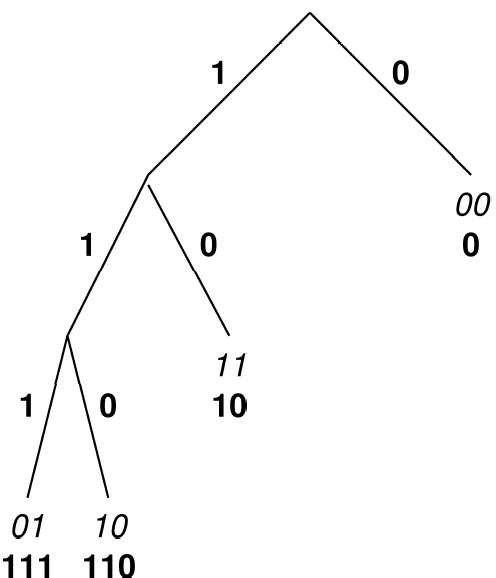
\includegraphics[scale=0.1]{figure1.png}%
%  		\caption{Baum}\label{fig:baum}%
%  	\end{center}%
% \end{figure}
%
% \begin{table}[h]%
%  	\begin{center}%
% 		\caption{Beispieltabelle}\label{tab:example}%
% 	 	\begin{tabular}{c|c}%
%  			Spalte1 & Spalte2\\
%  			\hline
%  			0 & 1\\
%  		\end{tabular}%
%  	\end{center}%
% \end{table}

% can use a bibliography generated by BibTeX as a .bbl file
% standard IEEE bibliography style from:
% http://www.ctan.org/tex-archive/macros/latex/contrib/supported/IEEEtran/bibtex
\bibliographystyle{IEEEtran}
% argument is your BibTeX string definitions and bibliography database(s)
\bibliography{IEEEabrv,references}





% \begin{figure}[h]%
%  	\begin{center}%
%  		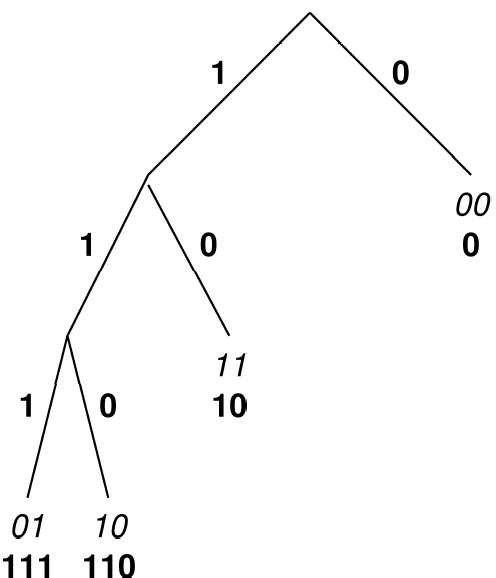
\includegraphics[scale=0.1]{figure1.png}%
%  		\caption{Baum}\label{fig:baum}%
%  	\end{center}%
% \end{figure}
%
% \begin{table}[h]%
%  	\begin{center}%
% 		\caption{Beispieltabelle}\label{tab:example}%
% 	 	\begin{tabular}{c|c}%
%  			Spalte1 & Spalte2\\
%  			\hline
%  			0 & 1\\
%  		\end{tabular}%
%  	\end{center}%
% \end{table}

% % can use a bibliography generated by BibTeX as a .bbl file
% % standard IEEE bibliography style from:
% % http://www.ctan.org/tex-archive/macros/latex/contrib/supported/IEEEtran/bibtex
% \bibliographystyle{IEEEtran}
% % argument is your BibTeX string definitions and bibliography database(s)
% \bibliography{IEEEabrv,references}



\section{Pascal GP100 Whitepaper}
The Tesla P100 has 5.3TFLOPS of FP64 performance, double as much (10.6 TFLOPS) of FP32, and four times as much (21.2 TFLOPS) of FP16.
The 16-bit floating point precision ability is though for Deep Learning.
Deep Learning does not require higher precision and this brings both higher speed and higher available storage for bigger models.

\subsection{Microprocessor architecture}
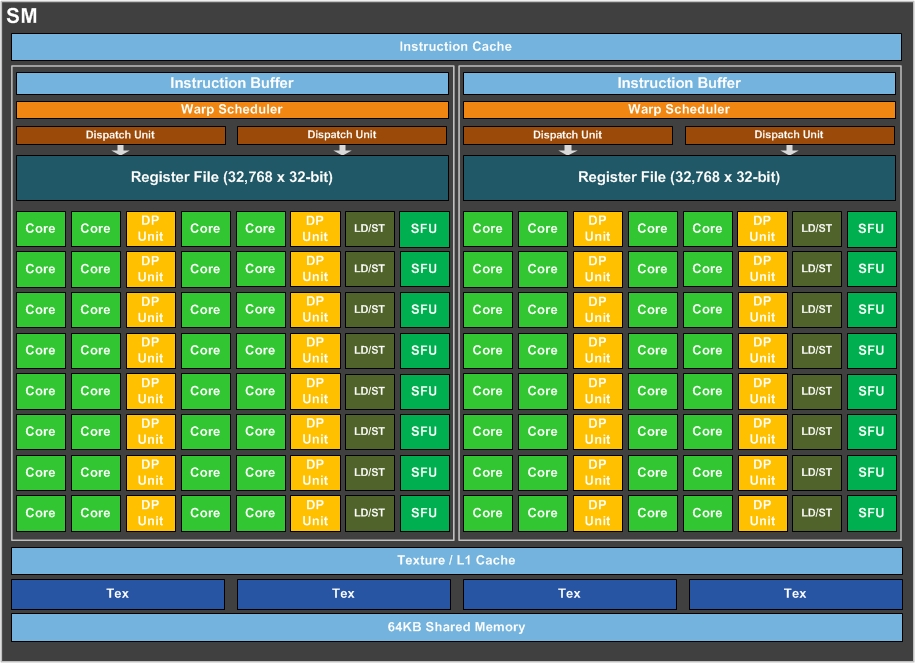
\includegraphics[width=0.9\linewidth]{gp100_sm}
\subsubsection{Processor structure}
It is composed of an array of GPCs, formed by TPCs, consisting of 2 SMs with 64 CUDA FP32 Cores and 4 texture units each.
The GP100 processor has 6 GPCs with 10 SMs each.
This makes a total of 3840 CUDA Cores
4 of the SMs on the chip are turned off, giving a total of 56 available SM units.

Each SM has 32 FP32 CUDA Cores, an instruction buffer, and a warp scheduler with two dispatch units.
Since the register file size per CUDA Core is doubled, there can be more thread blocks running concurrently.

The scheduler data path is changed with respect to Kepler and Maxwell.
A big improvement in the scheduler in comparison to Maxwell is that each warp scheduler can dispatch two warp instructions per clock.
This allows up to \textbf{TODO: What does UP TO mean?} twice FP16 throughput vs FP32.
There is also a 2:1 ratio of FP64 to FP32 CUDA Cores per SM, which now works better with the data path.
\subsubsection{Memory hierarchy}
Same as before

\subsubsection{On-chip memory}
The L1/shared memory structure has not changed since Maxwell.
Each SM has 64KB of shared memory (up to 32KB per Thread Block), with an additional L1/texture cache.
This improves on the 64KB configurable shared memory/L1 cache of Fermi and Kepler.

There are eight 512-bit memory controllers to communicate with off-chip memory.
There is a unifed 4096KB L2 cache, which gives 512KB per memory controller.

\subsubsection{Off-chip memory HBM2}
Each stack of HBM2 is controlled by a pair of memory controllers.
Stacked memory uses less surface, which allows denser servers.
A HBM2 stack is composed by 4 or 8 dies with microscopic wires which go down the stack.
Each HBM2 die has a 8Gb capacity, giving a total of 4 or 8GB per stack.
The stacks have to be connected to the chip via a passive silicon interposer.
The height of the dies is adjusted (the top die is thicker) in order to make good contact with the heat sink.
HBM1 supported only 4 dies per stack and 2Gb per die.
HBM1 supported 125GB/sec per stack while HBM2 supports 180GB/sec.
% P100 will have initially 4-die HBM2 stacks, making a total of 16GB of mmemory.
HBM2 has native support for ECC.
Error correction is important when large clusters or long application executions make errors likely.
ECC detects and corrects single-bit soft errors before they affect the system.
GDDR5 does not have internal ECC, which only allows ECC to detect error on the bus.
This additionally requires allocating a 6.25\% of the memory for error correction, and results in a 12-15\% reduction in bandwidth.

There is a new block on the chip called High-Speed Hub (HSHUB) which has access to the High-Speed Copy Engines enabling NVLink access.

\subsection{Compute Capability}
The minimum block size remains of 32 threads.
\subsubsection{Unified Memory Analysis \cite{li2015evaluation}}
An evaluation of Unified Memory as of GK110 is provided in \cite{li2015evaluation}.
It describes the Unified Memory programming model and presents an evaluation methodology to try to understand how the automatic system works.
It is known that the system handles data migration transparently, but the workflow is unknown.
They work on the K40 GPU and the Jetson TK1.
The latter is interesting because it has physically unified memory.
To evaluate the performance they use three different benchmarks.
One is the Matrix Multiplication benchmark.
It gets tested on both cuBLAS and a block matrix multiplication that uses shared memory.
Another is the Diffussion 3D Benchmark.
The last one is the Parboil Benchmark Suite, created for studying the performance of computer architectures and compilers.
Only the benchmarks using a constant memory size are used.
The tool used to analyze the different runs is the NVIDIA Profiler.
The comparison is made by modifying them to use Unified Memory.
No other optimization changes are made.
It is shown that the structure and content of PTX codes (pseudo-asssembly codes for CUDA) does not change.

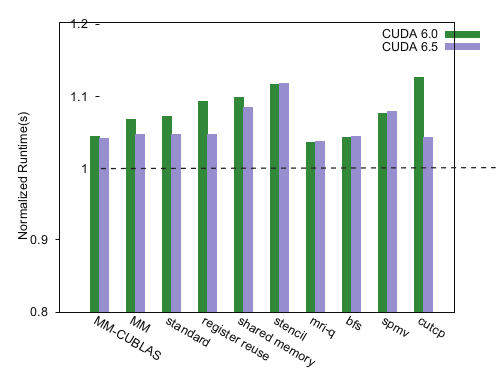
\includegraphics[width=0.9\linewidth]{unified_memory_benchmark_results}

They find that there are 10\% performance losses in average.
It is due to redundant memory transfers and page caching fault.
These losses are in some benchmarks considerably smaller under CUDA 6.5 than under CUDA 6.0.
The kernel running time in CUDA 6.5 does not improve.
It is the performance of launching and synchronizing what improves.
Interestingly, the TK1 uses the memory of CPU and GPU separately, even when it is physically one, resulting in uneeded copies.
It is also seen that pinned memory is used for Unified Memory.
It is revealed by the fact that copying times from host to device are much lower under Unified Memory.

Finally, five micro-benchmarks are created to look for the conditions causing the performance loss.
It is seen that memory is copied from host to device even if no kernel uses it.
Memory also gets copied back and forth even if it is only read by the GPU.
Only in the case that the CPU never reads or writes the data, are there no redundant memory transfers.

This same research group intends to analyze the performance under of Unified Memory in multi-GPU systems in the future.

\subsubsection{Unified Memory}
CUDA 4 introduced Unified Virtual Addressing.
UVA enabled pinning CPU memory to be accesible directly over PCIe without a memcpy.
This provided convenience but no performance.

Unified Memory was introduced in CUDA 6.
A single pointer referred to both CPU and GPU memory.
It worked through automatical data migration handled by software.
As described above, all managed memory touched by the CPU had to be synchronized.
Additionally, CPU and GPU could not access the same memory allocation simultaneously.
The address space was limited to the size of the GPU physical memory.

Now a single memory address space for CPU and GPU with 49-bit virtual addressing has been introduced.
Since current CPUs have up to 48-bit virtual addressing, this is enough to cover both spaces as a single virtual address space.
Now the memory limits of the GPU do not restrict the virtual space size.
Additionally, GP100 has hardware support for page faulting, which allows transparent access to data anywhere in the virtual address spaces.
This means there is no need for synchromization of all managed memory allocations.
The large address space allows direct addressing of very large datasets, much larger than the system memory.
Faulted pages are automatically migrated.
Mapping on access can sometimes be faster than migration (\textbf{TODO: When?})
CPUs can also fault and migrate memory from GPU.
CPU can even access data while a GPU kernel is running.
Coherency in this case could not be guaranteed in previous architectures.
Note that correct synchronization has to be taken care of as in any other parallel application.

Operating system support is being developed to enable GPUS to access memory allocated with the default OS allocator (such as malloc).

Aside from making GPU programming easier, this also allows easier use of C++ classes on GPU.
Any nested data can be automatically accessed thanks to the single virtual addres.

\subsubsection{Compute Preemption}
GP100 has preemption at instruction-level.
This is an improvement on block-level preemption of the Maxwell and Kepler architectures.
It allows interaction with long computing tasks, swapping contexts to GPU DRAM.
Otherwise, long running tasks can end up being killed by the OS or the CUDA driver.
Additionally, if a GPU is being used for display graphics and CUDA tasks, long running tasks can result in an unresponsive GUI.
This also makes interactive debugging work better.
Interactive debugging on Kepler and Maxwell required adding instrumentation during compilation to allow completion of thread blocks after an interrupt.
GP100 debugging is more robust and lightweight.


\subsection{Data transfer}
GPUDirect was introduced in Kepler allowed RDMA, lowering CPU overhead.
It enabled DMA, this means the CPU does not have to copy the data in its own memory.
It also enabled P2P data transfer between GPUs.
GPUDirect badnwidth is doubled in GP100.

Clusters of multi-GPU systems are being interconnected with InfiniBand(R) and 100Gb Ethernet.
The GPUs to CPUs ratio is increasing.
Fast cluster interconnections and this increasing ratio were causing PCIe to become a bottleneck.
That is why NVLink was introduced.
\subsubsection{NVLink}
Allows GPU-to-GPU data transfers.
It uses the new NVHS interconnect.
It is compatible with the GPU ISA, supporting shared memory multiprocessing.
Programs can execute directly on memory of another GPU with full capability.
Data is transmitted over a set of differential pairs with a bandwidth of 20Gb/sec each.
A total of 16 form a Link, with 8 pairs for each direction.
This gives a total bidirectional bandwidth of up to 40GB/sec
Since the GP100 supports up to 4 links, this allows up to 160GB/sec bidirectional data transfer.
PCIe Gen 3 x16, the largest in common use even though the standard is defined up to x32, provides a bandwidth of up to 31.75GB/s
A couple of GP100 cards can be connected with a bandwidth of up to more than 5x that of PCIe.

The NVLink controller is formed by a Pysical Layer, a Data Link Layer, and a Transaction Layer.
The package sizes range from 1 to 18 128-bit flits.
\textbf{TODO:}
The clock runs a t 1.25GHz.
It uses an embedded clock used at the received to capture data.
The Physical Layer takes care of deskewing across lanes, framing, scrambling/descrambling, polarity inversion and lane reversal.
% Polarity inversion and lane reversal allow for effective PCB routing.
The Data Link Layer is responsible for reliable transmission.
Packets are protected with a 25-bit CRC [\textbf{TODO}].
It is calculated over the current header and the previous payload.
It allows detection of up to 5 random bit errors or up to 25-bit bursts of errors on any lane.
Packets are stored in a replay buffer until the receiver acknowledges them.
If the transmitter times out waiting for acknowledgment, it starts retransmitting.

The Transaction Layer cares for synchromization, link flow control, virtual channels.
It can also aggregate multiple links together to provide higher communication bandwidth.

\subsection{TODOs}
\begin{itemize}
    \item Infiniband vs 100Gb Ethernet
\end{itemize}

% \begin{figure}[h]%
%  	\begin{center}%
%  		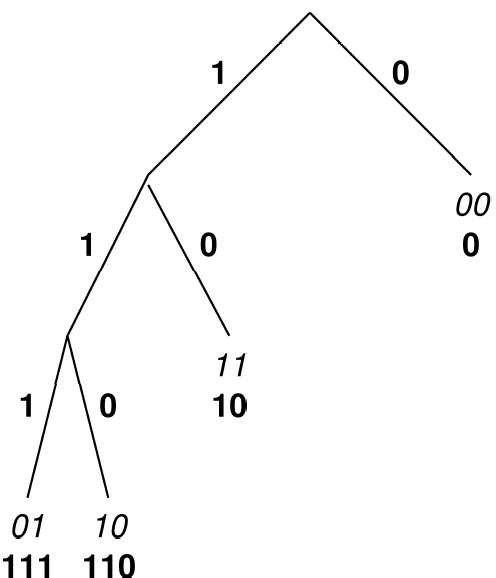
\includegraphics[scale=0.1]{figure1.png}%
%  		\caption{Baum}\label{fig:baum}%
%  	\end{center}%
% \end{figure}
%
% \begin{table}[h]%
%  	\begin{center}%
% 		\caption{Beispieltabelle}\label{tab:example}%
% 	 	\begin{tabular}{c|c}%
%  			Spalte1 & Spalte2\\
%  			\hline
%  			0 & 1\\
%  		\end{tabular}%
%  	\end{center}%
% \end{table}

% % can use a bibliography generated by BibTeX as a .bbl file
% % standard IEEE bibliography style from:
% % http://www.ctan.org/tex-archive/macros/latex/contrib/supported/IEEEtran/bibtex
% \bibliographystyle{IEEEtran}
% % argument is your BibTeX string definitions and bibliography database(s)
% \bibliography{IEEEabrv,references}



\section{Zusammenfassung und Ausblick}
blabla

\section{Glossary}

\textbf{SM} Streaming Multiprocessor \\
\textbf{SIMT} Single Instruction Multiple Threads \\
\textbf{TMU} Texture Mapping Unit \\
\textbf{ROPs} Raster Operations Pipelines (render output unit) \\
\textbf{LSU} Load/store Units \\
\textbf{SFU} Special Function Units \\
\textbf{GPC} Graphics Processing Cluster \\
\textbf{TPC} Texture Processing Cluster \\
\textbf{RDMA} Remote Direct Memory Acess \\
\textbf{ECC} Error Correcting Code \\
\textbf{NVHS} NVIDIA's High-Speed Signaling interconnect \\
\textbf{Flit} Flow control digit \\
\textbf{CRC} Cyclic Redundancy Check \\
\textbf{UVA} Unified Virtual Addressing \\
\textbf{ISA} Instruction Set Architecture \\
% \textbf{}  \\


%%%%%%%%%%%%%%%%%%%%%%%%%%%%%%%%%%%%%%%%%%%%%%%%%%%%%%%%%%%%%%%%%%%%%%%%%%
% 	Acknowledgements
%%%%%%%%%%%%%%%%%%%%%%%%%%%%%%%%%%%%%%%%%%%%%%%%%%%%%%%%%%%%%%%%%%%%%%%%%%

%\section*{Acknowledgment}
%\addcontentsline{toc}{section}{Acknowledgment}

%%%%%%%%%%%%%%%%%%%%%%%%%%%%%%%%%%%%%%%%%%%%%%%%%%%%%%%%%%%%%%%%%%%%%%%%%%
% 	References
%%%%%%%%%%%%%%%%%%%%%%%%%%%%%%%%%%%%%%%%%%%%%%%%%%%%%%%%%%%%%%%%%%%%%%%%%%

% trigger a \newpage just before the given reference
% number - used to balance the columns on the last page
% adjust value as needed - may need to be readjusted if
% the document is modified later
%\IEEEtriggeratref{8}
% The "triggered" command can be changed if desired:
%\IEEEtriggercmd{\enlargethispage{-5in}}

% references section
% NOTE: BibTeX documentation can be easily obtained at:
% http://www.ctan.org/tex-archive/biblio/bibtex/contrib/doc/

% can use a bibliography generated by BibTeX as a .bbl file
% standard IEEE bibliography style from:
% http://www.ctan.org/tex-archive/macros/latex/contrib/supported/IEEEtran/bibtex
\bibliographystyle{IEEEtran}
% argument is your BibTeX string definitions and bibliography database(s)
\bibliography{references}
%
% <OR> manually copy in the resultant .bbl file
% set second argument of \begin to the number of references
% (used to reserve space for the reference number labels box)
%\begin{thebibliography}{1}
%
%\bibitem{ref:kopka}
%H.~Kopka and P.~W. Daly, \emph{A Guide to {\LaTeX}}, 3rd~ed.\hskip 1em plus
%  0.5em minus 0.4em\relax Harlow, England: Addison-Wesley, 1999.
%
%\end{thebibliography}

%%%%%%%%%%%%%%%%%%%%%%%%%%%%%%%%%%%%%%%%%%%%%%%%%%%%%%%%%%%%%%%%%%%%%%%%%%
% 	End of the document
%%%%%%%%%%%%%%%%%%%%%%%%%%%%%%%%%%%%%%%%%%%%%%%%%%%%%%%%%%%%%%%%%%%%%%%%%%

\end{document}
